%!TEX root = ../Main.tex

\chapter{Vulkan Development Environment}
\label{cha:EnvSetup}
  \todo[inline]
  {
    High level goals of this chapter:\\
    -- Generating `vulkan.h'\\
    -- LunarG SDK\\
    -- Installing layers\\
    -- Present most important layers / extensions\\
  }
  \todo[inline]
  {
    Buzzwords: Tools, development environment, Vulkan in practice
  }

  % This chapter is a guide to setting up a Vulkan development environment in the context of \gls{ccpp} on a \gls{windows} operating system.

  % As can be expected, the steps required to setup a Vulkan environment depend on the development platform of choice.

  This chapter describes some practical aspects of Vulkan development and acts as a guide in setting up a Vulkan development environment. As can be expected, the steps required for such a setup depend on the kind of platform to be developed on.

  \todo[inline]{Mention differences on Linux and maybe other dev platforms.}

  \section{Hardware Vendor Support}
  \label{sec:HardwareVendorSupport}
    When setting up a development environment, one must first ensure that the hardware offers Vulkan support.

    Using and developing Vulkan applications requires support from the hardware. Information about Vulkan support for a particular piece of hardware can usually be found in the manual or the hardware vendor website. There are also third-party resources that can be consulted to check whether a particular piece of hardware provides Vulkan support. The \textit{Vulkan Hardware Database}\cite{vulkangpuinfo} is one such resource. This database even provides an overview of the supported hardware features and device extensions. In order to support Vulkan, hardware vendors have to provide driver implementations for the platform the user is targeting.

    \todo[inline]{No end-user support for Intel devices. \cite{intelvulkandriversonwindows}}

    \todo[inline]{Explain \acrfull{icd} here.}


  \section{Vulkan Header}
  \label{sec:VulkanHeader}
    Once it has been made sure that the current platform supports Vulkan,

    The Vulkan \gls{ccpp} header file is actually generated from a more abstract representation called the Vulkan API Registry. The most recent version can be found in the Vulkan-Docs repository on GitHub, which can be found in the Khronos Vulkan Registry\cite{vulkanregistry}. This repository contains the generated \gls{ccpp} header file. It also contains the file \lstinline{vkspec.xml} and a set of tools to generate the Vulkan header from it. The \lstinline{vkspec.xml} essentially contains annotated C code with XML markup that is easier to parse than pure C code. The annotations also contain contextual information, something pure C code could not easily or conveniently provide. This additional layer of abstraction was created in order to support generating a Vulkan API for contexts different from C and \gls{cpp}. This means that it is possible to use these tools to generate native bindings for other programming languages, such as \gls{csharp}, or \gls{python}.


  \section{Vulkan Common Loader}
  \label{sec:VulkanLoader}
    \todo[inline]{How to handle overlapping topics discussed earlier, e.g. layers and extensions?}

    \begin{figure}
      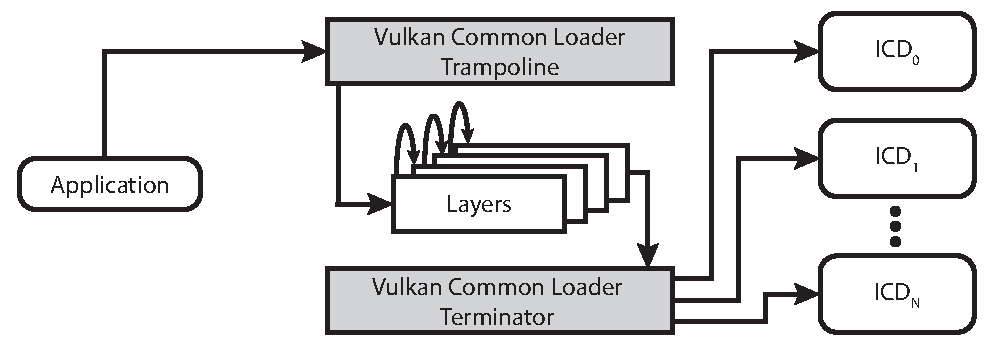
\includegraphics{Main/Images/VulkanLoaderInstanceLayers}
      \centering
      \caption{Communication between the application and the \glspl{icd} via the Vulkan Common Loader when using instance-level API calls.}
      \label{fig:VulkanLoaderWithInstanceLayers}
    \end{figure}

    \begin{figure}
      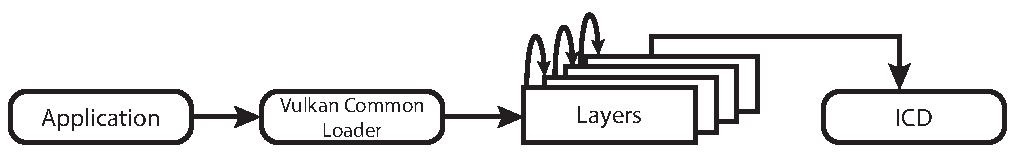
\includegraphics{Main/Images/VulkanLoaderDeviceLayers}
      \centering
      \caption{Communication between the application and an \gls{icd} via the Vulkan Common Loader when using device-level API calls.}
      \label{fig:VulkanLoaderWithDeviceLayers}
    \end{figure}

    The \textit{Vulkan Common Loader}, is an open source project mainly developed and maintained by the Khronos Group. It can be found in the Khronos Vulkan Registry\cite{vulkanregistry}. It is written in \gls{c} and can be used by application developers either as a static or dynamically linked library.

    The \textit{Vulkan Common Loader} is the interface between Vulkan applications and \glspl{icd}. It ensures that multiple \glspl{icd} can be installed on the same system without interfering with each other. It is also responsible for managing optional modules, called \textit{layers}. There are explicit and implicit layers. Explicit layers are only loaded when the Vulkan application requests these layers explicitly. This is done when creating a Vulkan instance or a Vulkan device. Implicit layers, on the other hand, are activated by default. An example for an explicit layer is some kind of validation layer, for instance one that tracks Vulkan object lifetimes. An exaple for an explicit layer is one that tracks the lifetimes of Vulkan objects.

    \todo{Explain layers here now?? Maybe merge sec \ref{sec:EnvLayersAndExtensions} with this one.}




  \section{Layers and Extensions}
  \label{sec:EnvLayersAndExtensions}
    \tbd
    \todo[inline]{Merge with the previous chapter?}


  \section{LunarG Vulkan SDK}
  \label{sec:LunarGSDK}
    The LunarG Vulkan \acrshort{sdk}\cite{lunargvulkansdk} is a \acrfull{sdk} developed by LunarG. LunarG is a software company that develops tools and infrastructure for Vulkan development. The company itself is sponsored by Valve Corporation. The first version of the LunarG \gls{sdk} was released at the same time as version 1.0 of the Vulkan specification.

    Developing a Vulkan application does not require the LunarG \gls{sdk} to be installed. For that, only the Vulkan header and common loader are required. However, the LunarG \gls{sdk} includes these two components and a number of additional components. These components are meant to help making it easier to develop Vulkan applications. Aside from the Vulkan header and the common loader, the \gls{sdk} also includes several Vulkan layers, debugging tools, tools that aid in creating shader modules compatible with Vulkan, the Vulkan API documentation, and a range of Vulkan samples and demos as well as a sample-driven tutorial.


  \section{Shaders}
  \label{sec:EnvShaders}
    As mentioned in section~\ref{sec:Pipelines} Vulkan expects shaders to be in \gls{spirv} format. Since \gls{spirv} is a binary format, it is meant to be the result of some kind of conversion operation from some other kind of shader representation. A common way to write shaders for Vulkan applications is by first writing them in \gls{glsl} and then converting these shaders to \gls{spirv} using a special tool. This tool is called \textit{Glslang}\cite{glslangrepo} and is a command-line based tool that is able to validate \gls{glsl} code and to convert it into other representations. \todo{Describe what exactly is required. layout=N, binding=N, set=N, \#extensionm, ...}It requires the \gls{glsl} source code to be written in a specific way in order to be converted to \gls{spirv}.

    \begin{lstlisting}[label=lst:glslangcmd]
glslangValidator -V Shader.vert -o Vertex.spv
glslangValidator -V Shader.frag -o Fragment.spv\end{lstlisting}

    Listing \ref{lst:glslangcmd} shows how to convert two shader programs, provided in \gls{glsl} format, to \gls{spirv} using Glslang. The \lstinline{-V} switch tells Glslang to convert to Vulkan-compatible \gls{spirv} format. The \lstinline{-o} switch is used to control how the output file is named. In the first line, the input is the file called \lstinline{Shader.vert} and the output is a file called \lstinline{Vertex.spv}, which will be in \gls{spirv} format. The second line does the same transformation for the input file \lstinline{Shader.frag} and the output file \lstinline{Fragment.spv}.

    Another approach is to use a custom-made fron-end that would be convertible to \gls{spirv}. This might be the favorable approach for many graphics or game engines since these technologies \todo{Do I need references here?}usually have their own abstract representation of shader functionality. Being able to directly translate to \gls{spirv} removes the need to translate into some human-readable form first, such as \gls{glsl}.


  \section{Debugging and Profiling}
  \label{sec:DebuggingAndProfiling}
    \todo[inline]{Describe debugging here.}

    Once a Vulkan application is running correctly, the developer might also be interested whether it runs \textit{efficiently}. This is especially important for many real-time applications such as video games. Due to the young age of Vulkan, there aren't many profiling tools specifically tailored to Vulkan applications. There are some tools that can aid in this regard, though. The LunarG SDK, as described in \ref{sec:LunarGSDK}, offers an API tracing and playback tools. This tool effectively records which commands are performed by an application, measuring the execution time of individual commands. This can help in tracking down bottlenecks observed on the host-side. The RenderDoc Graphics Debugging\cite{renderdoc} also has the capability of trascking API calls. However, these kinds of tools are not capable of capturing how the GPU behaves for a given Vulkan Application. At the time of writing, no Vulkan-specific GPU profiling tool is known to the author of this work. There other tools that are more general that can be used for GPU profiling, though. One such tool is NVIDIA FCAT\cite{nvidiafcat}. This tool requires a special piece of hardware, called a \textit{capture card}, that captures the output of a graphics card and displays analysis results directly on the attached computer display.

    \todo[inline]{Not many tools are there for profiling. Vulkan is still young.}
